\documentclass[a4paper,11pt]{article}
\usepackage{amsmath,amsthm,amsfonts,amssymb,amscd,amstext,vmargin,graphics,graphicx,tabularx,multicol} 
\usepackage[francais]{babel}
\usepackage[utf8]{inputenc}  
\usepackage[T1]{fontenc} 
\usepackage{pstricks-add,tikz,tkz-tab,variations}
\usepackage[autolanguage,np]{numprint} 
\usepackage{calc}

\setmarginsrb{1.5cm}{0.5cm}{1cm}{0.5cm}{0cm}{0cm}{0cm}{0cm} %Gauche, haut, droite, haut
\newcounter{numexo}
\newcommand{\exo}[1]{\stepcounter{numexo}\noindent{\bf Exercice~\thenumexo} : }
\reversemarginpar

\newcommand{\bmul}[1]{\begin{multicols}{#1}}
\newcommand{\emul}{\end{multicols}}

\newcounter{enumtabi}
\newcounter{enumtaba}
\newcommand{\q}{\stepcounter{enumtabi} \theenumtabi.  }
\newcommand{\qa}{\stepcounter{enumtaba} (\alph{enumtaba}) }
\newcommand{\initq}{\setcounter{enumtabi}{0}}
\newcommand{\initqa}{\setcounter{enumtaba}{0}}

\newcommand{\be}{\begin{enumerate}}
\newcommand{\ee}{\end{enumerate}}
\newcommand{\bi}{\begin{itemize}}
\newcommand{\ei}{\end{itemize}}
\newcommand{\bp}{\begin{pspicture*}}
\newcommand{\ep}{\end{pspicture*}}
\newcommand{\bt}{\begin{tabular}}
\newcommand{\et}{\end{tabular}}
\renewcommand{\tabularxcolumn}[1]{>{\centering}m{#1}} %(colonne m{} centrée, au lieu de p par défault) 
\newcommand{\tnl}{\tabularnewline}

\newcommand{\trait}{\noindent \rule{\linewidth}{0.2mm}}
\newcommand{\hs}[1]{\hspace{#1}}
\newcommand{\vs}[1]{\vspace{#1}}

\newcommand{\N}{\mathbb{N}}
\newcommand{\Z}{\mathbb{Z}}
\newcommand{\R}{\mathbb{R}}
\newcommand{\C}{\mathbb{C}}
\newcommand{\Dcal}{\mathcal{D}}
\newcommand{\Ccal}{\mathcal{C}}
\newcommand{\mc}{\mathcal}

\newcommand{\vect}[1]{\overrightarrow{#1}}
\newcommand{\ds}{\displaystyle}
\newcommand{\eq}{\quad \Leftrightarrow \quad}
\newcommand{\vecti}{\vec{\imath}}
\newcommand{\vectj}{\vec{\jmath}}
\newcommand{\Oij}{(O;\vec{\imath}, \vec{\jmath})}
\newcommand{\OIJ}{(O;I,J)}


\newcommand{\reponse}[1][1]{%
\multido{}{#1}{\makebox[\linewidth]{\rule[0pt]{0pt}{20pt}\dotfill}
}}

\newcommand{\titre}[5] 
% #1: titre #2: haut gauche #3: bas gauche #4: haut droite #5: bas droite
{
\noindent #2 \hfill #4 \\
#3 \hfill #5

\vspace{-1.6cm}

\begin{center}\rule{6cm}{0.5mm}\end{center}
\vspace{0.2cm}
\begin{center}{\large{\textbf{#1}}}\end{center}
\begin{center}\rule{6cm}{0.5mm}\end{center}
}



\begin{document}
\pagestyle{empty}
\titre{Séance d'AP 2 : Ecritures scientifiques d'un nombre}{}{}{3ème}{}

\vspace*{0.2cm}

\setlength{\fboxrule}{2pt}
\begin{flushleft}
\framebox{\begin{minipage}{\linewidth}

\vspace*{0.2cm}

\underline{\textbf{{\large Rappels de cours}}}\\

\textbf{Définition :} L'écriture scientifique d'un nombre décimal est l'unique écriture de ce nombre sous la forme $a \times 10^{n}$, où:
\bi
\item $a$ est un nombre décimal compris entre 1 et 10, 10 étant exclu ;
\item $n$ est un nombre entier relatif (positif ou négatif).\\
\ei
\vspace*{0.2cm}

\textbf{Exemples :}  $2,145 \times 10^{5}$ est l'écriture scientifique du nombre 214 500\\
 \hspace*{ 1.8cm}               $1,25 \times 10^{-2}$  est l'écriture scientifique du nombre 0, 0125



\vspace*{0.2cm}
\end{minipage}}
\end{flushleft}

\vspace*{0.4cm}

\bmul{2}
\exo \\
Ecrire les nombres suivants sous forme de puissance de 10. \\



\noindent 1 000 = . . . . . . . . .\\
100 000 000 = . . . . . . . \\
0,0000001 = . . . . . . . . \\
0,1 = . . . . . . . . . \\
0,001 = . . . . . . . . . . .\\
 

\columnbreak

\exo \\
Associer les écritures scientifiques avec les nombres auxquels elles correspondent. \\



\noindent $2,718 \times 10^{3}$ \hspace*{2cm} 2,718\\
$2,718 \times  10^{0}$    \hspace*{2cm} 2 718\\
$2,718 \times  10^{2}$    \hspace*{2cm} 27,18\\
$2,718 \times  10^{1}$    \hspace*{2cm} 27 180\\
$2,718 \times  10^{5}$   \hspace*{2cm} 271,8\\
$2,718 \times  10^{-2}$   \hspace*{1.8cm} 0,02718\\



\emul

\exo \\
Donner l'écriture décimale de chaque nombre. 

\bmul{2}

$A = 1,35 \times 10^{5}$\\


$W = 45 200 \times 10^{-5}$\\


$B = 0,05  \times 10^{4}$\\


\columnbreak

$K = 0,006 05 \times 10^{2}$\\


$C =2 \times 10^{-4}$\\


$X = 13,45 \times 10^{-3}$\\

\emul

\exo \\
Écrire les nombres suivants à l'aide de l'écriture scientifique. \\

\bmul{2}

$M = 789 \times 10^{4}$\\

$R = 0,67 \times 10^{-3}$\\


$G = 645,3 \times 10^{-15}$\\





\columnbreak

$L = 0,003 \times 10^{6}$\\

$S = 12,8 \times 10^{-1}$\\


$D = 0,056 \times 10^{17}$\\

\emul






\exo \\
Voici les distances entre le soleil et les planètes du systèmes solaire :  

\renewcommand{\arraystretch}{1.5}

\begin{center}
\begin{tabular}{|c|c|}
\hline 
Vénus : 105 millions km &  Mercure : $58 \times 10^{6}$ km \\ 
\hline 
Mars : $2 250 \times 10^{5}$ km &  Terre : $15 \times 10^{7}$ km \\ 
\hline 
 Uranus : 2 880 millions km & Saturne : 1 425 000 000 km \\ 
\hline 
Jupiter : 780 000 000 km &  Neptune : $45 \times 10^{8}$ km \\ 
\hline 
\end{tabular}
\end{center}

\q Ranger ces distances par ordre croissant (attention pour les comparer il faut les écrire à l'aide de l'écriture scientifique).\\

\q Compléter alors les légendes ci-dessous.
\begin{center}
\includegraphics[scale=0.95]{systemesolaire.eps} 
\end{center}


\vspace*{0.5cm}

\exo \\
Donner l'écriture scientifique puis l'écriture décimale des expressions suivantes.

\bmul{3}

$T = \dfrac{8 \times 10^{4} \times 7 \times 10^{2}}{14 \times 10^{-3}}$\\

\columnbreak


$J = \dfrac{2 \times 10^{5}\times 9 \times 10^{-4}}{15 \times 10^{5}}$\\

\columnbreak

$H = \dfrac{4\times 10^{-6} \times 3 \times 10^{-2}}{6 \times 10^{-5} \times 5 \times 10^{2}}$\\

\emul  

\vspace*{0.3cm}

\exo \\

Un vaisseau spatial a mis 20 ans pour faire le voyage planète X-Terre.\\ Sachant que la planète X est située à 4,5 années lumière de la Terre et qu'une année-lumière est égale à $9,5 \times 10^{12}$ km, calculer la vitesse moyenne de ce vaisseau spatial exprimée en km par an. On donnera l'écriture scientifique du résultat.\\

\vspace*{0.3cm}

\exo \\

En informatique, on utilise comme unités de mesure les multiples de l'octet :

\begin{center}
$1 ko = 10^{3}$ octets, \hspace*{0.3cm} $1 Mo = 10^{6}$ octets,  \hspace*{0.3cm} $1 Go = 10^{9}$ octets.
\end{center}


\begin{center}

\includegraphics[scale=0.7]{disquedur.eps} 

\end{center}

\textbf{Contenu du disque dur externe :}
\bi
\item 1 000 photos de 900 ko chacune ;
\item 65 vidéos de 700 Mo chacune\\
\ei






  $\rightarrow $ \textbf{L'affirmation suivante est-elle vraie} : le transfert de la totalité du contenu du disque dur externe vers l'ordinateur n'est pas possible.\\



\end{document}
